\section{PROCEDURES}

\subsection{Mission join procedure}

At the end of the briefing the Mission Commander will announce "Next step,
flight comms check" or words to that effect, which is the signal to join the
server and start ground power and report in on the briefed Flight frequency as
soon as is feasible. If there is anything required about which server slot, it
should have been provided in the briefing.

No permission from Control is required to start up engines. No move before
Taxi. Generally, the order is:

\narrow{%

  \begin{orderedlist}

    \item Enter server slot

    \item Start ground power

    \item Connect Air supply (AWG-9 cooling)

    \item Formation Lights on, Nav lights per SOP (see 4.3)

    \item Tune radios, Forward Radio for internal comms, aft Radio for ATC

    \item Perform Flight comms check

    \item Continue start-up

  \end{orderedlist}
}

\subsection{CV Ops}

Please refer to \href
  {https://cloud.132virtualwing.org/s/wSMBb66EEEJztNW}
  {132\nd Carrier Operations 132-TTP-19}

\subsection{Aircraft Light Configurations}

\subsubsection{CV Daytime}

All lights \textbf{off} for Departure and Recovery

\subsubsection{CV Night-time}

All lights \textbf{off} always except.

\begin{itemize}
  \setlength\parskip{0pt}

  \item Lights all on steady when ready to launch except Landing lights (they
    remain off)

  \item When Landing, all lights Landing lights on + flashing, but extinguished
    immediately on arrestment

  \item NVG's not to be used during Cat Launch or landings

\end{itemize}


\subsubsection{Airfield Day and Night}

\begin{itemize}
  \item Navigation lights on Flash and set to steady when ready for taxi.

  \item Anti-collision strobe off on the ground and enabled immediately prior
    to entering the runway.

  \item Taxi lights off when stationary and enabled immediately prior and
    during taxi.

  \item After landing and vacating the runway, the Anti-Collision beacon must
    be turned OFF. Check taxi lights are on.
\end{itemize}

The lighting configuration is changed when holding short and after exiting the
runway.

\subsubsection{Interior lighting}

The lighting required for optimal NVG use is very low, especially on the VDI,
it will be unreadably low. For the HUD, less reflection is seen in NVG if using
the daytime green filter, rather than red. Elsewise lighting as desired, noting
that the ACM panel is on the right side for Pilot.


\subsection{INS procedures}

The Tomcat INS is prone to degrade. Planning INS updates is part of the mission
planning process for the MC. Visual fixes are the most reliable, although we
have tables for TACAN updates which are tested to be more inaccurate than we
hoped.

For visual fixes, flyover points should be found that have straight lines to
lead in, approached from a specific angle as to present an easier fix point and
cross referenced across canopy sight lines, perhaps with wingman help.

Care should be taken in making low level passes under 14,000 feet AGL in enemy
territory.

INS updates must be done before and after critical actions and at least once
per hour of flight time. Coast lines are best, hit at 90 degrees.

\subsection{NVG constraints and process}

NVG's require very turned down lighting in the cockpit but are quite useful for
spotting things on the ground. Green Hud is preferable to Red Hud with NVG's.

Landing and departing with NVG's equipped is prohibited under normal
circumstances due to ejection safety requirements (neck injury due to weight).

After takeoff and prior to landing, NVG's can be unstowed and used as required.

\subsection{Fuel efficiency}

  Available Fuel is a combat resource. The availability of fuel allows for

  \begin{itemize}

    \item Prolonged on station times and VUL

    \item Lifesaving use of high-power settings on demand

    \item Lifesaving combat effectiveness in ACM and BVR

  \end{itemize}

  Procedures should be followed to ensure optimal fuel use throughout all
  phases of execution including:

  \begin{itemize}

    \item Non-emergency Afterburner usage

    \item General throttle settings

    \item Cruising Altitude

    \item Climb and descent profiles

  \end{itemize}

\sidebyside{0.77}{%

    In general, all Pilots should avoid Afterburner and consider it an
    emergency or combat only tactic. Additionally, care should be taken to use
    conservative fuel flow as soon as is practically possible and plan altitude
    and missions accordingly.

    The default loadout by 108\th will always be to include extra fuel tanks
    unless specified and retain them.

    The Tomcat comes with two reminders for best climb speed and best cruise
    speed.  These are marked on the AoA indexer. The {\color{red}Red} mark is
    the optimal climb and max endurance AoA at 8.5 units. The
    {\color{blue}Blue} mark at 5 units is the cruise AoA, for max range.
}{%
  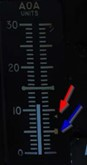
\includegraphics[width=\textwidth,align=t]{fuel-flow}%
}

\sidebyside{0.6}{%
  A clean Tomcat at 20,000 feet ASL can cruise at 1000-1500 lbs Fuel Flow per
  engine which equates to 0.48M and 220kts A fully laden Tomcat can cruise at
  2000-2500 at 30,000MSL at 0.60M. It takes longer to find the pure speed and
  slow down than we will encounter in a normal 2-3 hour session. Pure cruising
  speed will give us over 6 hours flight time.

  Therefore, the easiest way to consolidate this information is to set a
  reasonable Fuel Flow first since we should always have more fuel than we need
  for a gaming session. Setting 2000 per engine gives us 5hrs of cruise at many
  different altitudes for around 220 kts.

  It was noted that in testing Altitude had minimal effect on fuel efficiency
  for the Tomcat over 15000 feet ASL, only really on speed. Its stores layouts
  aren't draggy like on the Hornet either, so for endurance purposes you will
  gain far more from actually handling the throttle gently, performing good
  climbs, not letting the AoA hit over 10 so the Maneuvering flaps kick in and
  the speed is hampered, and so on. We are also unlikely to get a benefit on
  the long loiter times either, due to combat performance demanding use of
  Afterburner (to get a good shot) being a more preferable and useful Combat
  strategy.
}{%
  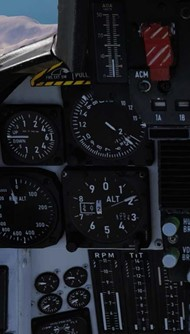
\includegraphics[width=\textwidth,align=t]{fuel-endurance}%
}
